\textbf{Mindmap}
Es wurde ein Brainstorm zu den Branchenspezifischen Herausforderungen und M�glichkeiten durchgef"uhrt. Das Ergebnis ist in der folgenden Mindmap dargestellt.\\

\begin{figure}[h!]
	\centering
	\caption{Mindmap Mobile Banking}
		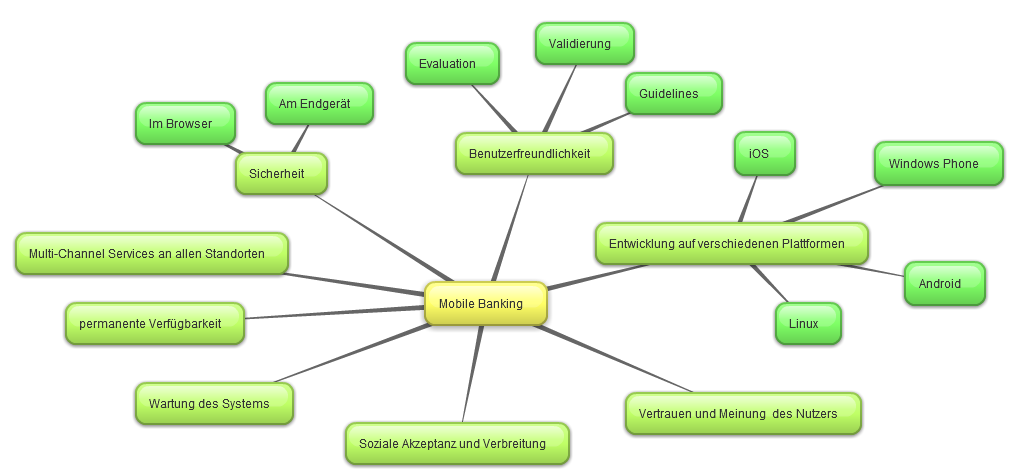
\includegraphics[width=16cm, height=10cm]{figures/mm_mobilebanking}
\end{figure}

\begin{figure}[h!]
	\centering
	\caption{Mindmap Cloud Computing}
		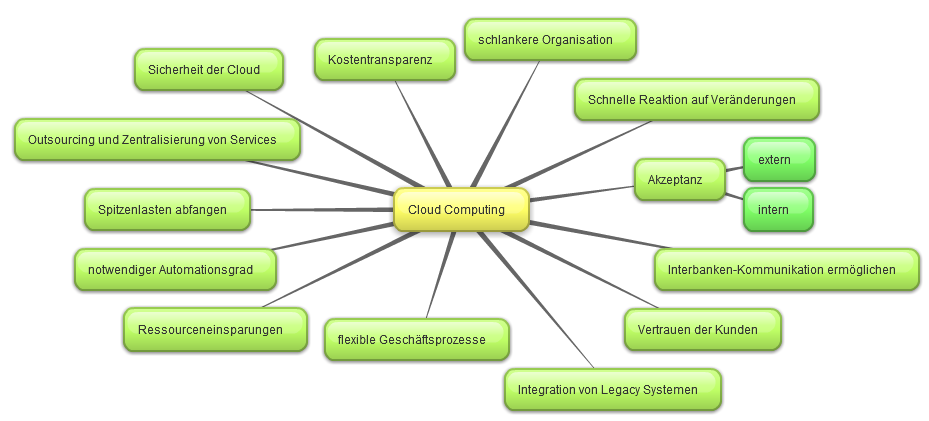
\includegraphics[width=16cm, height=9cm]{figures/mm_cloudcomputing}
\end{figure}

\begin{figure}[h!]
	\centering
	\caption{Mindmap Contactless Payment}
		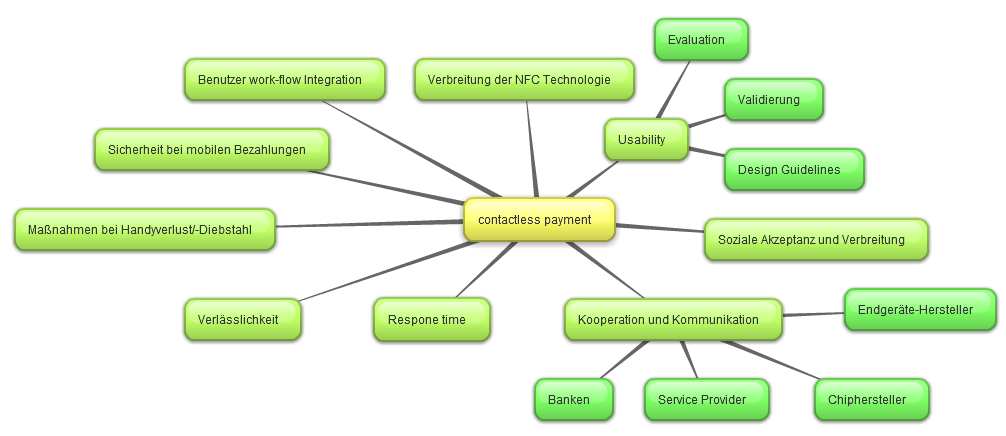
\includegraphics[width=16cm, height=9cm]{figures/mm_contactlesspayment}
\end{figure}

\newpage
\textbf{Vision \& Ziele}\\
Auf Basis der gefundenen Herausforderungen f�r das Unternehmen wurden die folgenden vier Ziele definiert welche mit einer IT-Strategie erreicht werden sollen. 

\begin{enumerate}
	\item Mobiles und intuitives Banking f�r die Kunden, anywhere and anytime.

	\item Wirtschaftliche und flexible Verwaltung von internen und externen Business-Prozessen und Produkten. 
	
	\item Aktualit"at und Innovationsf"uhrerschaft durch die Bezahltechniken von Morgen.
	
	\item Vertrauensbildung bei Kunden und Mitarbeitern zu allen Innovationen und Produkten.
	
\end{enumerate}

\textbf{Generelle Strategien}
\begin{enumerate}

	\item Einrichtung eines modernen \textit{Multi-Channel Banking}, das es den Kunden erm�glicht, im Sinne der \textit{Self-Service Technology} orts- und zeitungebunden auf personalisierte, intuitive Services zuzugreifen.

	\item B"undelung von Kerngesch"aft, Kernprozessen und Kern-Knowhow. Einheitlicher unternehmensweiter Einsatz. wirtschaftliches Management von Supportprozessen. Forcieren von standortspezifischen Spezialisierungen.

	\item Verfolgung und Absch"atzung von Trends und Entwicklungen sowohl im Payment-Bereich als auch in der IT mit Unterst�tzung eines weltweit renommierten IT Consultingunternehmen. Evaluation und Beobachtung neuer technischer Entwicklungen in Kooperation mit dem Beraterunternehmen. Teilnahme bzw. Mitarbeit an relevanten Industrie-Konsortien aus dem Payment-Bereich.

	\item Sicherheit, Verf"ugbarkeit und Verl"asslichkeit in allen Systemen.\\
F�r eine Bank ist es wichtig ihre Finanztransaktionen und -dienstleistungen m�glichst sicher durchzuf�hren. Daf�r ist es notwendig die Systeme der Bank schon bei der Entwicklung so zu gestalten, dass es zu keinem Fehlverhalten w�hrend dem produktiven Einsatz kommen kann.

\end{enumerate}









